\chapter{共有三階層LSTMによる生活パターン発見と状態推定}
\label{chap:model}

同じ「勉強・研究」という活動名でも、文章を書く時間と実験装置を操作する時間では、観測される入力行動や生活情報が異なる。一方、場所が変わっただけで同じ作業を別の行動とみなすことも適切ではない。固定カテゴリによる活動分類と、個人固有のタスク推定を並行して行うと、何を別の状態として識別するかが二重に定義される。

本研究の提案構成では、活動の意味カテゴリをあらかじめ24個に固定せず、共有の時系列表現から拠点と行動パターンを扱う。現在・日次の5尺度も同じエンコーダから推定する。行動候補の発見、本人による同一性の確認、名前の付与は別の操作である。特徴が似た観測のまとまりが得られても、そのまとまりを直ちに「修論執筆」などの意味へ置き換えない。

対応する実装は\texttt{life-discovery-v1}である。24クラス分類を含む従来のHierarchicalLSTMと、独立したContextLSTMは比較条件として保持するが、提案構成と同時に二重の行動推定を行うものではない。実参加者における有効性は第\ref{chap:evaluation}章の評価課題であり、以下の数理的定義と実装の対応を、推定性能の検証とは分けて記述する。

\section{推定対象と観測情報}
\label{sec:prediction-targets}

参加者\(p\)について、イベント発生時刻と受信時刻の双方が推定時刻\(t\)以下である観測の集合を\(\mathcal H_p^{\rm obs}(t)\)とする。入力\(x_{p,d,u,k}\in\mathbb R^{98}\)は、33個の観測値、対応する33個の存在指示、32次元の文章特徴からなる。\(d\)は日、\(u\)は日内区間、\(k\)は区間内ビンを表す。観測値の欠測と実測ゼロを区別し、文章特徴はローカルで生成する。

本人の活動回答、拠点・行動確認、モデル推定を観測特徴にしない。24活動の回答は入力区間の境界にも用いない。入力系列を構成するTimelineには観測記録だけを渡し、質問の回答内容を変えただけで同じ観測系列の表現が変わることを防ぐ。

数式中の入力\(x\)は前処理後の特徴とする。33観測値の平均と標準偏差は訓練側の観測済み座標だけから求め、標準化後も欠測座標を存在指示でゼロ化する。存在指示と文章32座標は標準化しない。文章特徴はローカルSentenceTransformerで生成した文埋め込みを固定ランダム射影したものであり、エンコーダの同一性をcheckpointと照合する。文エンコーダの導入・比較条件は§\ref{sec:sentence-encoder}に示す。

共有エンコーダの出力を現在表現\(C_p(t)\in\mathbb R^{48}\)と日次表現\(D_p(t)\in\mathbb R^{48}\)とし、推定対象を次式で表す。

\[
\left(z_p^{P}(t),z_p^{B}(t),\hat y_p^{\rm cur}(t),\hat y_p^{\rm day}(t)\right)
=f_\theta\left(\mathcal H_p^{\rm obs}(t)\right).
\]

\(f_\theta\)はパラメータ集合\(\theta\)を持つ共有エンコーダと各出力層を合わせた写像である。\(z^P,z^B\in\mathbb R^{32}\)はそれぞれPlaceとBehaviorの表現であり、32種類の場所・行動を意味しない。\(\hat y^{\rm cur},\hat y^{\rm day}\in[1,5]^5\)は現在・日次の尺度予測ベクトルで、5尺度の順序は気分、疲労、ストレス、集中度、眠気に固定する。尺度は本人回答に対応する研究上の推定対象であり、診断や客観的な心理状態の測定ではない。

Placeは本人が区別する生活拠点、Behaviorは本人固有の行動パターンである。同一場所の別作業と、別場所の同じ作業を独立に確認できるよう、両軸のIDを分離する。既存APIの\texttt{task}および\texttt{taskCheck}はBehaviorの互換名として維持し、第三の推定対象は作らない。

\section{三階層の時間表現}

各階層には隠れ次元48の単方向LSTMを一つずつ用いる。LSTMの基本更新はゲートを介したセルの保持と更新である\autocite{hochreiter1997lstm}。本実装で用いる忘却ゲートはLSTMの後の発展に対応する\autocite{gers2000forget}。階層を\(\ell\in\{\mu,m,M\}\)とし、順にMicro、Meso、Macroを表す。階層内の時刻添字を\(j\)、入力を\(v_j^\ell\in\mathbb R^{d_\ell}\)、隠れ状態とセル状態を\(h_j^\ell,c_j^\ell\in\mathbb R^{48}\)とする。入力次元は\(d_\mu=98\)、\(d_m=d_M=48\)である。各階層のゲート更新を次式で定義する。

\[
\begin{aligned}
i_j^\ell&=\sigma(W_i^\ell v_j^\ell+U_i^\ell h_{j-1}^\ell+b_i^\ell),&
f_j^\ell&=\sigma(W_f^\ell v_j^\ell+U_f^\ell h_{j-1}^\ell+b_f^\ell),\\
o_j^\ell&=\sigma(W_o^\ell v_j^\ell+U_o^\ell h_{j-1}^\ell+b_o^\ell),&
g_j^\ell&=\tanh(W_g^\ell v_j^\ell+U_g^\ell h_{j-1}^\ell+b_g^\ell),\\
c_j^\ell&=f_j^\ell\odot c_{j-1}^\ell+i_j^\ell\odot g_j^\ell,&
h_j^\ell&=o_j^\ell\odot\tanh(c_j^\ell).
\end{aligned}
\]

\(i_j^\ell,f_j^\ell,o_j^\ell\in(0,1)^{48}\)は入力・忘却・出力ゲート、\(g_j^\ell\in(-1,1)^{48}\)はセルへ書き込む候補である。\(\sigma(a)=1/(1+\exp(-a))\)と\(\tanh\)は各座標へ適用し、\(\odot\)は要素積を表す。ゲート種別\(\gamma\in\{i,f,o,g\}\)ごとに、\(W_\gamma^\ell\in\mathbb R^{48\times d_\ell}\)は入力重み、\(U_\gamma^\ell\in\mathbb R^{48\times48}\)は再帰重み、\(b_\gamma^\ell\in\mathbb R^{48}\)はバイアスである。実装の入力側・再帰側バイアスは式の\(b_\gamma^\ell\)へ合算して表す。したがってMicroでは98次元の観測を、MesoとMacroでは48次元の下位表現を、同じ形式のゲートで48次元の記憶へ更新する。重みは階層別に持ち、PlaceとBehaviorごとに別の三階層を作るものではない。

入力ゲートは候補情報の書込み、忘却ゲートは過去セルの保持、出力ゲートは隠れ状態への読出しを制御する。これらのゲートは学習されるため、時間尺度ごとの固定平滑化係数ではない。セルの加法的経路は記憶の保持を助けるが、長期依存を常に学習できることを保証しない。

\subsection{MicroとMeso}

以下では同一参加者の推定を記述するため、参加者添字\(p\)と推定時刻\(t\)を必要な箇所以外で省略する。Microは正時境界で区切った最大1時間を、最大12個の5分ビンとして処理する。末尾の短いビンは実際の長さで構成し、推定時刻より後の観測を含めない。日\(d\)の区間\(u\)における有効ビン数を\(K_{d,u}\)とする。Microのゲート式に\(v_k^\mu=x_{d,u,k}\)を代入し、区間ごとの初期状態を\((h^\mu_{d,u,0},c^\mu_{d,u,0})=(0,0)\)として順に更新する。区間の最終隠れ状態\(w_{d,u}\in\mathbb R^{48}\)は

\[
w_{d,u}=h^\mu_{d,u,K_{d,u}}
=\operatorname{LastHidden}\left(\operatorname{LSTM}_{\mu}(x_{d,u,1:K_{d,u}})\right)
\]

である。\(\operatorname{LastHidden}\)はパディングを除いた系列の最終隠れ状態を返す操作、\(1:K_{d,u}\)は最初から有効長までの系列を表す。Mesoは日\(d\)の有効区間数\(U_d\)に対して\(v_u^m=w_{d,u}\)を入力し、\((h^m_{d,0},c^m_{d,0})=(0,0)\)から時間順に更新する。日表現\(q_d\in\mathbb R^{48}\)は

\[
q_d=h^m_{d,U_d}
=\operatorname{LastHidden}\left(\operatorname{LSTM}_{m}(w_{d,1:U_d})\right)
\]

である。保存テンソルは一日48区間を上限とし、有効長を別に保持する。提案構成では活動回答による追加分割を行わない。過去日はその日の終端まで、当日は推定時刻までの観測を使う。過去日の観測でも、受信が推定時刻に間に合っていることを要求する。

実装は有効長の系列をパックし、パディングを無操作の実測ビンとしてLSTMへ与えない。長さゼロの保存区間の表現はゼロとする。ちょうど日付が変わった時点には空の部分ビンを一つ設け、有効長を扱えるようにする。推定時刻が区間途中であれば、その時点までの部分系列の最終状態を使うため、区間終了後の情報を待ってから現在予測を行う構成ではない。

\subsection{Macroと融合}

当週は日本標準時の月曜日開始とする。当週開始前に対応する28個の日別観測特徴\(r_i\in\mathbb R^{98}\)を古い順に線形射影し、当週の日表現列へ時間方向に連結する。\(r_i\)にも第\ref{chap:observations}章の訓練側統計による前処理を適用する。過去28日は保存されたMesoの隠れ状態ではなく、日別観測を再集約した特徴である。当週開始を\(W\)とすると、履歴窓は\((W-(i+1)\text{日},W-i\text{日}]\)、\(i=27,\ldots,0\)である。下式の\(r_1\)は\(i=27\)の最古窓、\(r_{28}\)は\(i=0\)の最新窓に対応する。右閉区間であるため、\(W\)ちょうどのイベントは最後の履歴窓に含まれる。受信締切はいずれの窓でも推定時刻\(t\)である。

推定時刻が属する当週の日添字を\(d_*\)、当日の現在区間添字を\(u_*\)とする。当週の日は古い順に\(1,\ldots,d_*\)と数える。履歴の射影行列とバイアスを\(W_H\in\mathbb R^{48\times98}\)、\(b_H\in\mathbb R^{48}\)とし、Macroの入力\(v_j^M\)を次式で定義する。

\[
v_j^M=
\begin{cases}
W_Hr_j+b_H,&1\le j\le28,\\
q_{j-28},&29\le j\le28+d_*.
\end{cases}
\]

Macroは\((h^M_0,c^M_0)=(0,0)\)から上記のゲート式を\(28+d_*\)ステップ適用する。その最終隠れ状態\(H\in\mathbb R^{48}\)は

\[
H=h^M_{28+d_*}
=\operatorname{LastHidden}\left(\operatorname{LSTM}_{M}
\left([W_Hr_1+b_H,\ldots,W_Hr_{28}+b_H,q_1,\ldots,q_{d_*}]\right)\right).
\]

となる。日次表現\(D\in\mathbb R^{48}\)と現在表現\(C\in\mathbb R^{48}\)は次式で得る。

\[
D=\tanh(W_D[q_{d_*};H]+b_D),\qquad
C=\tanh(W_C[w_{d_*,u_*};D;H]+b_C).
\]

\(W_D\in\mathbb R^{48\times96}\)、\(W_C\in\mathbb R^{48\times144}\)は融合行列、\(b_D,b_C\in\mathbb R^{48}\)はバイアスである。\([\cdot;\cdot]\)は特徴方向の連結であり、Macro式中の列は時間方向の連結である。実装の\texttt{top\_day}が\(D\)、\texttt{top\_work}が\(C\)に対応する。

\subsection{階層間の状態の受渡し}

時間方向の状態更新と階層間の受渡しを区別するため、階層\(\ell\)のゲート式全体を写像\(\Phi_\ell\)と表す。下位の最終隠れ状態が上位の一入力となる関係は、次式にまとめられる。

\[
\begin{aligned}
(h^\mu_{d,u,k},c^\mu_{d,u,k})
&=\Phi_\mu(x_{d,u,k},h^\mu_{d,u,k-1},c^\mu_{d,u,k-1}),\\
(h^m_{d,u},c^m_{d,u})
&=\Phi_m(w_{d,u},h^m_{d,u-1},c^m_{d,u-1}),\\
(h^M_j,c^M_j)
&=\Phi_M(v_j^M,h^M_{j-1},c^M_{j-1}).
\end{aligned}
\]

Microのセル\(c^\mu\)は区間内の記憶であり、Mesoへ渡す\(w_{d,u}\)はその読出しである。同様に、Mesoのセル\(c^m\)をMacroへ移すのではなく、日表現\(q_d\)を入力する。したがって三階層のセルは互いに独立した48次元の記憶を持ち、下位の細かな系列を上位の時間単位へ要約する。逆方向には\(H\)と\(D\)を融合式へ渡し、現在表現\(C\)を文脈で条件付ける。上位の文脈はMicroのセルへ直接注入しない。

現行実装は各系列を初期状態から再計算する。推論間のhidden/cell持越しや、本番のTBPTTによる逐次重み更新は含まない。条件付き状態保持を行う比較計画の切断長と保存・復元規則は§\ref{sec:legacy-ssl-and-adaptation}で定義する。表現の受渡し、LSTM内部状態の持越し、離散状態IDの時間遷移はそれぞれ異なる操作であり、最後の時間遷移は§\ref{sec:pattern-discovery}のグラフとして扱う。

\section{拠点・行動・主観尺度の出力}

PlaceとBehaviorは共通の現在表現から別の射影を通して得る。\(W_P,W_B\in\mathbb R^{32\times48}\)は軸別の射影行列、\(b_P,b_B\in\mathbb R^{32}\)はそのバイアスである。任意のベクトル\(v\)について\(\operatorname{norm}(v)=v/\max(\lVert v\rVert_2,\epsilon)\)、\(\epsilon=10^{-12}\)とすれば、

\[
z^P=\operatorname{norm}\{\tanh(W_PC+b_P)\},\qquad
z^B=\operatorname{norm}\{\tanh(W_BC+b_B)\}.
\]

射影後の\(\tanh\)は座標の大きさを制限し、正規化前のノルムが\(\epsilon\)以上なら、正規化後の内積をコサイン類似度として比較できる。文章特徴の32次元化は凍結した固定射影であるのに対し、この二つの\(48\to32\)射影は共有エンコーダとともに学習する。入力文章の32次元と出力の32次元は、座標の意味や重みを共有しない。極小ノルムによる正規化の例外はマップ入力時に再検査する。

現在・日次の尺度は別の出力層で推定する。\(W_{\rm cur},W_{\rm day}\in\mathbb R^{5\times48}\)と\(b_{\rm cur},b_{\rm day}\in\mathbb R^5\)をそれぞれ尺度出力の重みとバイアスとすると、

\[
\hat y^{\rm cur}=1+4\sigma(W_{\rm cur}C+b_{\rm cur}),\qquad
\hat y^{\rm day}=1+4\sigma(W_{\rm day}D+b_{\rm day}).
\]

となる。右辺の定数1は5座標へ加え、各尺度の出力を本人回答の1〜5の範囲へ写す。Place・Behaviorは現在表現\(C\)から、日次尺度は日次表現\(D\)から得るため、日次尺度を現在尺度の単純平均として定義しない。

5尺度の予測値を行動クラスタリングの距離へ連結しない。この構成は、出力得点の変化だけによって直接別の行動ノードへ割り当てることを避ける。ただしエンコーダは共有されるため、行動表現から心理状態の影響が完全に除去されるわけではない。

同様に、射影を二つ設けるだけでは場所と行動の意味は分離されない。自宅でしか行わない作業は、自宅を示す観測と共起し続ける。両者を区別するための情報は、異なる場所で同じ行動を行った観測、同じ場所で別行動を行った観測、および独立した本人確認である。観測上区別できない状態は不明のまま残す。

\section{自己教師あり学習と本人確認の併用}
\label{sec:joint-learning}

学習は自己教師あり損失と本人回答の損失を同時に最適化する。別段階の事前学習を必須とする構成ではない。教師がない観測からも表現を学習するが、無回答を架空の正解として補わない。

\subsection{マスク再構成と将来予測}

非空のバッチを\(\mathcal B\)、その件数を\(n_{\mathcal B}=|\mathcal B|\)とし、例\(i\in\mathcal B\)の最新有効ビンを\(x_i\in\mathbb R^{98}\)とする。以下の添字\(j\)はこの最新ビンの特徴座標である。基礎量の座標集合を\(\mathcal J_v=\{1,\ldots,33\}\)、文章座標集合を\(\mathcal J_e=\{67,\ldots,98\}\)とする。基礎量のうち時間周期、区間長、heartbeat鮮度、収集設定の座標集合を\(\mathcal J_{\rm ex}\subset\mathcal J_v\)とし、これらは再構成対象から除外する。文章長\texttt{text\_chars}の基礎量座標を\(j_{\rm text}\in\mathcal J_v\)、基礎量\(j\)の元の存在指示を\(m_{i,j}\)とする。元の観測有効性\(\omega_{i,j}\)を

\[
\omega_{i,j}=
\begin{cases}
m_{i,j},&j\in\mathcal J_v\setminus\mathcal J_{\rm ex},\\
m_{i,j_{\rm text}},&j\in\mathcal J_e,\\
0,&\text{その他}
\end{cases}
\]

と定義する。座標34〜66のpresence自体は予測の正解にしない。観測済みの基礎量ごとに独立な選択変数\(\xi_{i,j}\sim\operatorname{Bernoulli}(0.2)\)を抽選し、文章には例ごとに一つの\(\xi_i^{\rm text}\sim\operatorname{Bernoulli}(0.2)\)を抽選する。\(\operatorname{Bernoulli}(0.2)\)は確率0.2で1、それ以外で0を返す分布である。\(j\in\mathcal J_e\)では\(\xi_{i,j}=\xi_i^{\rm text}\)とし、対象外の座標では\(\xi_{i,j}=0\)とする。選択された有効座標集合は

\[
\mathcal M=
\{(i,j):i\in\mathcal B,\ \omega_{i,j}=1,\
\xi_{i,j}=1,\ x_{i,j}\text{が有限}\}
\]

である。基礎量を隠すときは値\(x_{i,j}\)と対応するpresence \(x_{i,33+j}\)をともに0にする。文章は32座標全体を一つのブロックとして隠す。マスク後の現在表現から元の特徴を再構成し、\(\mathcal M\)だけに損失を適用する。

文章ブロック自体の選択確率も0.2であり、32座標を独立に抽選してからブロックへ拡張する旧SSLの方式とは異なる。文章を隠すときは\texttt{text\_chars}の値と存在指示も消す。ただし文章長座標を\(\mathcal M\)へ含めるかは、その基礎量自身の抽選による。非マスク入力の出力を将来予測・関係・尺度・分散損失に用い、再構成だけにはマスク入力からの別の順伝播を用いる。例\(i\)のマスク後の現在表現を\(C_i^{\rm mask}\in\mathbb R^{48}\)とし、\(W_{\rm rec}\in\mathbb R^{98\times48}\)と\(b_{\rm rec}\in\mathbb R^{98}\)を再構成ヘッドの重みとバイアスとすると、\(\hat x_i=W_{\rm rec}C_i^{\rm mask}+b_{\rm rec}\)である。

\[
\mathcal L_{\rm rec}=\frac{\sum_{(i,j)\in\mathcal M}(\hat x_{i,j}-x_{i,j})^2}{\max(1,|\mathcal M|)}.
\]

再構成の正解は標準化後の元の最新ビンである。\(|\mathcal M|\)は有効座標数であり、集合が空の場合は損失を0とする。将来予測は64次元の\([z^P;z^B]\)から次の1時間\((t,t+1\text{時間}]\)の観測特徴を推定する。例\(i\)の予測時刻を\(t_i\)、1時間後の終端を\(t_i^+=t_i+1\text{時間}\)、当該分割の教師締切を\(T_i^{\rm split}\)、データ取得締切を\(T_{\rm acq}\)とする。将来教師を利用できる指示を

\[
\gamma_i^+=\mathbf1\{t_i^+<T_i^{\rm split},\ t_i^+\le T_{\rm acq}\}
\]

と定義する。将来区間の生特徴を訓練側統計で変換した教師を\(\tilde x_i^+\in\mathbb R^{98}\)とし、その区間の観測有効性\(\omega_{i,j}^+\)を\(\omega_{i,j}\)と同じ座標規則で求める。将来教師マスクは\(m_{i,j}^+=\gamma_i^+\omega_{i,j}^+\mathbf1[\tilde x_{i,j}^+\text{が有限}]\)である。\(W_+\in\mathbb R^{98\times64}\)と\(b_+\in\mathbb R^{98}\)を将来予測ヘッドの重みとバイアスとして、

\[
\hat x_i^+=W_+[z_i^P;z_i^B]+b_+,\qquad
\mathcal L_{\rm future}=\frac{\sum_{i,j}m_{i,j}^+(\hat x_{i,j}^+-\tilde x_{i,j}^+)^2}{\max(1,\sum_{i,j}m_{i,j}^+)}
\]

とする。和は\(i\in\mathcal B\)と\(j=1,\ldots,98\)について取り、有効でない座標は和から除く。将来損失には隠す座標の抽選を行わず、予測対象として有効な観測座標すべてを用いる。各損失は例ごとの平均をさらに平均するのではなく、バッチ全体の有効座標で平均する。予測対象の1時間の終端が分割の締切以上、またはデータ取得締切より後である場合は、そのターゲットを使わない。将来特徴はその終端までに受信された観測から作る教師であり、現在入力へ渡すものではない。この条件により、再構成は現在の観測間の関係、将来予測は次の1時間に関わる表現を学習する。

\subsection{本人確認による関係学習}

軸\(a\in\{P,B\}\)ごとに、例\(i\)で本人が確認した正規IDを\(k_i^a\)とする。ここでの添字\(i,j\)はともにバッチ内の例であり、特徴座標ではない。別名解決後の本人確認IDを双方が持つペア集合\(\mathcal P_a=\{(i,j):i,j\in\mathcal B,\ j<i,\ k_i^a,k_j^a\text{が有効}\}\)を作る。\(j<i\)によって各組を一度だけ数える。正規化された埋め込みの内積\((z_i^a)^\top z_j^a\)を類似度とし、同一IDの表現は近づけ、異なるIDは類似度が0.3を超える場合に離す。

\[
\ell_a(i,j)=
\begin{cases}
1-(z_i^a)^\top z_j^a,& k_i^a=k_j^a,\\
\max\{0,(z_i^a)^\top z_j^a-0.3\},& k_i^a\ne k_j^a,
\end{cases}
\qquad
\mathcal L_{\rm rel}^{a}=\frac{\sum_{(i,j)\in\mathcal P_a}\ell_a(i,j)}{\max(1,|\mathcal P_a|)}.
\]

\(\ell_a(i,j)\)は一組の関係損失、\(\mathcal L_{\rm rel}^a\)は有効ペア間の平均である。同一IDの項は類似度1で0になり、異なるIDの項は類似度0.3以下では0になる。異なるIDをすべて反対方向へ押し離す制約ではない。Placeの正解をTaskの違いから生成することも、その逆も行わない。未確認、わからない、移動中には同一性ラベルを作らない。命名だけの操作も同一性の教師を追加しない。

\subsection{尺度損失と全体損失}
\label{sec:scale-and-total-loss}

現在・日次の尺度には回答済み有限値の座標だけのHuber損失を用いる\autocite{huber1964robust}。scopeを\(s\in\{\mathrm{cur},\mathrm{day}\}\)、尺度添字を\(j=1,\ldots,5\)、例\(i\)に対応する本人回答を\(y_{i,j}^s\)とする。有効回答マスクを\(m_{i,j}^{y,s}=\mathbf1[y_{i,j}^s\text{が回答済みの有限値で }1\le y_{i,j}^s\le5]\)とし、有効な例と尺度の組を\(\mathcal O_s=\{(i,j):i\in\mathcal B,\ m_{i,j}^{y,s}=1\}\)とする。残差を\(r=\hat y_{i,j}^{s}-y_{i,j}^{s}\)、閾値1のHuber関数を\(\rho_1\)とすれば、

\[
\mathcal L_s=\frac{\sum_{(i,j)\in\mathcal O_s}\rho_1(\hat y_{i,j}^{s}-y_{i,j}^{s})}{\max(1,|\mathcal O_s|)},\qquad
\rho_1(r)=\begin{cases}\tfrac12r^2,&|r|<1,\\|r|-\tfrac12,&|r|\ge1.\end{cases}
\]

となる。残差の絶対値が1未満では二乗誤差、1以上では線形に増えるため、大きい残差の寄与を二乗誤差より抑える。未回答座標は補完せず、分母にも含めない。

埋め込みが単一の値へ縮退することを抑えるため、各軸にバッチ内分散のペナルティも加える。軸\(a\)の埋め込み座標\(j=1,\ldots,32\)について、バッチ平均を\(\bar z_j^a\)、母分散を\(V_j^a\)とすると、

\[
\bar z_j^a=\frac1{n_{\mathcal B}}\sum_{i\in\mathcal B}z_{i,j}^a,\qquad
V_j^a=\frac1{n_{\mathcal B}}\sum_{i\in\mathcal B}
(z_{i,j}^a-\bar z_j^a)^2
\]

である。\(n_{\mathcal B}\ge2\)の場合、分散損失を

\[
\mathcal L_{\rm var}^{a}=\frac1{32}\sum_{j=1}^{32}
\max\{0,0.05-\sqrt{V_j^a+10^{-4}}\}
\]

とする。0.05は各座標の標準偏差に対する下限、\(10^{-4}\)は平方根内の安定化定数である。\(V_j^a\)はバッチ件数で除した分散であり、不偏分散ではない。バッチが一例の場合、\(\mathcal L_{\rm var}^a=0\)とする。回答のない尺度損失と有効ペアのない関係損失もゼロとし、欠測を架空の教師に置き換えない。尺度損失は現在・日次ごとに有効座標で平均するため、一方の回答数の多さだけで他方を希釈しない。全体は次式である。

\[
\mathcal L=\mathcal L_{\rm rec}+\mathcal L_{\rm future}
+\mathcal L_{\rm cur}+\mathcal L_{\rm day}
+0.1\sum_{a\in\{P,B\}}\mathcal L_{\rm rel}^{a}
+0.1\sum_{a\in\{P,B\}}\mathcal L_{\rm var}^{a}.
\]

24クラスの交差エントロピーは含めない。分散項や関係損失は表現の制約であり、意味の分離を保証する定理ではない。既定の最適化はAdamW\autocite{loshchilov2019adamw}、学習率0.001、weight decay0.001、バッチ8、12エポック、乱数seed37、勾配ノルム上限1である。AdamWのweight decayは損失への単純なL2項の加算と区別する。観測例は各エポックでシャッフルし、LSTMの状態は例間で引き継がない。

再構成、将来予測、現在尺度、日次尺度の係数は各1であり、関係損失と分散損失の係数0.1はPlace・Behaviorのそれぞれに掛かる。全体損失\(\mathcal L\)の勾配は共有エンコーダへ集まり、再構成ヘッドには再構成項、将来ヘッドには将来項、各尺度ヘッドには対応する尺度項が伝わる。この同時最適化によって、観測の構造と本人の確認・回答を共通の時系列表現へ反映する。

\section{カテゴリ数を固定しないパターン発見}
\label{sec:pattern-discovery}

DiscoveryMapは、閾値に基づく逐次プロトタイプマップに、有向の時間遷移グラフを付したものである。プロトタイプの幾何学的な近さと、時間的に隣接した状態への変更を別々に記録する。ノード数はデータと本人確認に応じて変わり、24活動の数に拘束されない。

\subsection{プロトタイプ割当てと更新アルゴリズム}

軸\(a\in\{P,B\}\)のノードID集合を\(\mathcal V^a\)とし、ノード\(j\in\mathcal V^a\)に、代表ベクトル\(c_j^a\in\mathbb R^{32}\)、割当て件数\(n_j^a\in\mathbb N_0\)、本人確認の有無\(b_j^a\in\{0,1\}\)を保持する。\(\mathbb N_0\)は0以上の整数の集合である。プロトタイプ集合は\(\mathcal C^a=\{c_j^a:j\in\mathcal V^a\}\)、全ノード数は\(K_a=|\mathcal V^a|\)である。別名から正規IDを返す写像を\(\operatorname{can}_a\)とし、未知または未確認IDの欠如を\(\bot\)で表す。未確認候補数とその容量を

\[
K_{\rm unc}^a=\sum_{j\in\mathcal V^a}(1-b_j^a),\qquad
B_{\max}=256
\]

と定義する。この上限は未確認候補に適用し、本人確認済みのIDを含む全ノード数の上限とはしない。

アルゴリズムの入力は、訓練側の観測から固定したモデルで得る時刻順の組\((t_\nu,z_\nu^a,k_\nu^a)\)である。\(\nu\)は観測の処理順、\(t_\nu\)は割当て対象時刻、\(z_\nu^a\)は軸別埋め込み、\(k_\nu^a\)は訓練締切までに利用できる本人確認IDであり、確認がなければ\(\bot\)とする。全座標が有限で\(\lVert z_\nu^a\rVert_2>10^{-8}\)であることを検査し、マップ内で再正規化した\(\zeta_\nu^a=z_\nu^a/\lVert z_\nu^a\rVert_2\)を用いる。零ベクトル・極小ノルム・非有限値はエラーとする。代表も単位長なので、コサイン類似度と勝者は

\[
s_{\nu j}^a=(\zeta_\nu^a)^\top c_j^a,\qquad
j_\nu^*=\operatorname*{arg\,max}_{j\in\mathcal V^a}s_{\nu j}^a,\qquad
s_\nu^*=s_{\nu j_\nu^*}^a
\]

である。同点の場合はIDの順で決定する。\(\mathcal V^a=\varnothing\)なら\(j_\nu^*=\bot\)、\(s_\nu^*=-\infty\)とする。受入れ閾値を\(\tau=0.88\)とし、割当てID\(a_\nu\)を次式で定める。

\[
a_\nu=
\begin{cases}
\operatorname{can}_a(k_\nu^a),&k_\nu^a\ne\bot,\\
j_\nu^*,&k_\nu^a=\bot,\ s_\nu^*\ge\tau,\\
\operatorname{newID}_a(t_\nu),&
k_\nu^a=\bot,\ s_\nu^*<\tau,\ K_{\rm unc}^a<B_{\max},\\
\bot,&\text{その他}.
\end{cases}
\]

\(\operatorname{newID}_a(t_\nu)\)は当該軸と時刻から新候補の識別子を作る操作であり、固定活動番号を返すものではない。本人確認IDへの割当てを類似度より優先する第1分岐は、訓練側のマップ構築にだけ用いる。これを含む構築手順は次のとおりである。

\begin{enumerate}
\def\labelenumi{\arabic{enumi}.}
\item
  同一モデルで再符号化した既知IDの元観測をアンカーとして読み込み、代表\(c_j^a\)を初期化する。アンカーはIDに対応する元観測であり、旧モデルの重心ではない。アンカーの件数は\(n_j^a=0\)とする。確認済みアンカーを先に確保し、未確認アンカーには候補容量を適用する。
\item
  各\(t_\nu\)を厳密な昇順で処理し、上の割当て式を適用する。\(a_\nu=\bot\)なら代表を更新せず、時間辺を作るための直前割当てを消去して次へ進む。
\item
  \(a_\nu\notin\mathcal V^a\)なら、\(c_{a_\nu}^a=\zeta_\nu^a\)、\(n_{a_\nu}^a=0\)でノードを作る。本人確認IDの新規作成では\(b_{a_\nu}^a=1\)、新候補では0とする。確認済みIDは未確認候補の容量によって拒否しない。
\item
  割当て先\(j=a_\nu\)に次の再帰更新を適用し、本人確認があれば\(b_j^a=1\)とする。観測日と確認日も区別して記録する。
\item
  §\ref{sec:transition-graph}の条件で時間辺の回数を更新し、現在の割当てを次の直前割当てとして保持する。
\end{enumerate}

手順4の更新で用いる中間ベクトルを\(v_j^a=n_j^ac_j^a+\zeta_\nu^a\)とすると、

\[
c_j^a\leftarrow
\begin{cases}
v_j^a/\lVert v_j^a\rVert_2,&\lVert v_j^a\rVert_2>10^{-8},\\
\zeta_\nu^a,&\text{その他},
\end{cases}
\qquad n_j^a\leftarrow n_j^a+1
\]

である。新規ノードおよびアンカーは件数0で初期化するため、最初の割当てで代表はその埋め込みへ更新される。更新ごとに正規化するため、全埋め込みの単純な算術平均と同一ではなく、従来GrowingMapの欠測に応じた座標別平均（§\ref{sec:legacy-growingmap}）とも異なる。

上限時に十分近い代表がない観測は\(\bot\)となり、最寄りへ強制割当しない。本人確認済みのIDを候補数の上限だけで削除しない。本方式は閾値型の逐次プロトタイプ法であり、関連研究としてのGrowing Neural Gasの誤差蓄積、第2勝者や近傍の更新、辺の加齢・削除、誤差に基づく挿入則を実装したものではない。GNGとの相違と従来マップの数理は§\ref{sec:legacy-growingmap}および§\ref{sec:legacy-transition-ratios}に整理する。

\subsection{時間遷移グラフと推論時の固定}
\label{sec:transition-graph}

ここでは軸を\(\alpha\in\{P,B\}\)、辺の始点・終点IDを\(a,b\)と書き、軸とノードの添字を区別する。時間遷移グラフを\(\mathcal G^\alpha=(\mathcal V^\alpha,\mathcal E^\alpha,N^\alpha)\)とし、\(N_{ab}^\alpha\in\mathbb N_0\)を状態変更回数、\(\mathcal E^\alpha=\{(a,b):a\ne b,\ N_{ab}^\alpha>0\}\)を有向辺集合とする。回数はマップ再構築時に0から集計する。実装はPlaceとBehaviorの両マップに辺を持つが、生活パターンの提示にはBehaviorのマップを用いる。

軸ごとの直前割当てを\(\pi^\alpha=(a,t_{\rm prev})\)または\(\bot\)とし、最初は\(\bot\)とする。現在の割当てが\(b\)、時刻が\(t_\nu\)で、\(\pi^\alpha\ne\bot\)の場合の時間差を\(\Delta t=t_\nu-t_{\rm prev}\)と定義する。隣接した有効割当ての増分条件は

\[
N_{ab}^{\alpha}\leftarrow N_{ab}^{\alpha}
+\mathbf1\{a\ne b,\ 0<\Delta t\le1\text{時間}\}
\]

である。現在が未知なら\(\pi^\alpha\leftarrow\bot\)とし、辺を加えない。有効割当てなら、時間差が1時間を超えて辺を加えない場合も含めて\(\pi^\alpha\leftarrow(b,t_\nu)\)とする。この手順によって、長い未観測区間や候補上限による未知区間を跨いで辺を作らない。自己遷移は数えず、同じノードが続く場合にも直前時刻を更新する。

保存・表示する辺の量は回数であり、同一状態への滞在を含む次観測の遷移確率ではない。例えば\(a,a,b\)という系列では、\(a\)での滞在は辺を増やさず、時間条件を満たす\(a\to b\)だけを1回数える。従来構成の状態変更率\(Q_{ab}\)（§\ref{sec:legacy-growingmap}）と同様に、仮に変更回数から構成比を導出しても「記録された状態変更の内訳」である。従来の12時間という接続条件は新方式に流用しない。

マップ全体の保存状態を\(\mathscr M^\alpha\)とし、プロトタイプ、件数、確認属性、別名、時間辺の回数を含める。検証・テスト・ライブ推論で埋め込み\(z^\alpha\)を受け取るときは、同じ正規化と順位付けによる勝者\(j^*\)と最大類似度\(s^*\)を求め、候補IDを

\[
\hat k^\alpha=
\begin{cases}
j^*,&\mathcal V^\alpha\ne\varnothing,\ s^*\ge0.88,\\
\bot,&\text{その他}
\end{cases},
\qquad
(\theta,\mathscr M^\alpha)_{\rm after}
=(\theta,\mathscr M^\alpha)_{\rm before}
\]

とする。下付き\(\rm before,after\)は一回の推論の前後を表す。本人確認IDによる優先割当てはこの推論式には入れず、候補IDと正解IDを独立に比較できるようにする。新ノード生成、代表更新、件数加算、時間辺加算を推論時には行わない。類似度が閾値を満たしても、モデル推定として表示するにはさらに§\ref{sec:confirmation-and-estimation}の支持条件を必要とする。

マップの構築は訓練側データだけで行い、新しい候補の反映は次回のバッチ再学習時である。埋め込みが変わったときには、既知IDの元観測を新モデルで再符号化し、古い重心を新しい特徴空間へ混ぜない。離散状態IDの系列とその時間辺は、三階層LSTMが生成した表現を事後に割り当てたものであり、上位LSTMのセル状態そのものではない。

\section{意味付けと候補・推定の区別}
\label{sec:confirmation-and-estimation}

24活動の本人回答は、モデルとマップを固定した後に、対応する行動ノードの説明件数として集計する。一つのノードに複数の活動名が対応してよく、活動名の追加でノード数や重心を変えない。この集計は提案モデルの学習損失でも、別の24クラス予測器でもない。評価区間の注釈を用いて事前の対応表を作ることは避ける。

意味の命名と機械の推定は分けて保存する。例えば未確認候補に「修論執筆」と本人が命名した場合、その名称は本人による解釈であり、クラスタリングだけで自動獲得した意味ではない。場所や文章特徴だけから実際の作業を確定しない。

本人が対象区間のIDを確認した記録は\texttt{confirmed}、\texttt{source=self\_report}として扱う。これと、モデルが凍結マップへ割り当てた\texttt{candidate}、割当てに至らない\texttt{unknown}、表示条件を満たすモデル推定\texttt{estimated}、\texttt{source=model}を区別する。候補ノードが本人確認を持つことと、新しい区間のIDを本人が確認したことも同一ではない。本人確認表示とモデル推定の一致は評価対象であり、一方を他方へ自動変換しない。

ライブでIDを推定表示する初期条件は、本人確認の支持が2日以上、軸の検証が2件以上かつID一致率0.5以上、最大類似度0.88以上、次候補との差0.08以上である。単一候補の場合や、本人確認・統合が更新されて未学習の場合は断定しない。閾値は探索的設定で、コサイン類似度を校正された確率と解釈しない。

各尺度は学習10回答・検証3回答に満たない項目の数値を表示しない。未学習、推定時刻から遡って1時間以内に終了してその時刻までに受信されたセッションがない場合、将来時点で学習されたモデル、異なる文章エンコーダの利用も推定停止条件とする。heartbeatや開閉センサの周期観測だけでは、このセッションの鮮度条件を満たさない。確認質問の選択に用いる同日3時間の条件（§\ref{sec:context-confirmations}）によって、推論の1時間条件が緩和されることもない。これらの下限は表示を抑制する条件であり、精度保証ではない。

\section{検証・運用と従来構成の位置付け}
\label{sec:legacy-and-deployment}

\subsection{時系列分割と候補モデルの検証}

直近28日の観測から最大240時点を選び、最低12時点・3日を要求する。日単位の時系列順で約65\%を訓練、20\%を検証、15\%をテストとする。各分割にはその締切までに受信した教師だけを使う。本人回答時点の追加後に480時点を超える場合はエラーとし、黙って切り捨てない。正規化統計は訓練側だけで求める。

検証では将来特徴予測のマスク付き二乗誤差と、有効な現在・日次尺度のHuber損失の和を比較する。正規化が異なる候補モデルと現行モデルも、同じ検証時点・同じ誤差尺度へ戻して比較する。テスト成績をモデル昇格へ使わない。ID一致率や尺度別MAEも保存するが、提示された正解IDが少ないことを考慮して解釈する。

検証目的関数には再構成・関係・分散の各損失を加えない。各エポックの候補をこの目的関数で選び、適合する現行\texttt{life-discovery-v1}モデルがある場合には同じ検証集合で比較し、候補が悪化しない場合に昇格する。ここでの現行モデルとの比較は、従来の24活動分類器との研究上の比較とは異なる。テストは明示実行時だけ集計し、昇格へ用いない。

\subsection{方式選択と保存・提示}
\label{sec:runtime-selection}

新構成は\texttt{research\_architecture=discovery}として明示選択し、従来構成を\texttt{legacy}として保持する。現在・日次・拠点・行動を一つのcheckpointから推論し、独立ContextLSTMの学習ワーカーは起動しない。旧checkpoint、元データ、回答、命名を削除せず、保存先を分離する。後日の振り返りは再解析時刻とモデルIDを持つ別記録とし、当時のライブ推定を上書きしない。

サーバー設定の既定は\texttt{legacy}である。提案方式の学習では、従来方式とは別の\path{discovery/}保存先に候補・有効・旧版のcheckpointを保持する。CLIは単一参加者の完全なexportと、方式の由来を確認できる出力先を要求し、旧checkpointのディレクトリへ上書きしない。

新しい状態IDに基づく歩数基準と介入の検証は未完了である。このため、新構成では旧状態マップに依存する歩数保存・運動提案、および旧疲労推定に依存する提案判定を動かさない。5尺度の推定と候補の確認・命名・訂正は維持する。生活パターンが得られることと、それに基づく支援が有効であることは別の検証対象である。

% 追加: 従来breakCheckとlive時のDiscovery支援経路を区別する。
一方、LSTMとは別の\texttt{typing\_change}と本人の訂正理由を使う質問経路は新構成にも残る。質問予算を4枠より増やした場合、訂正率の変化に対する\texttt{typingReason}を選択できる。\texttt{discovery\_support\_mode}が\texttt{off}または\texttt{shadow}の場合、質問予算等の条件を満たすと、入力訂正の変化と直近2時間の\texttt{mistype}回答に基づく従来の\texttt{breakCheck}を選択できる。\texttt{live}ではこの従来提案を抑止し、Discoveryの支援判断と事前・事後評価を用いる別経路を選択する。既定4枠ではこれらのイベント質問を選択せず、22時以降は日次回答を優先する。この補助経路は新しいBehavior IDや5尺度推定の有効性に基づく支援ではなく、休憩提案がすべての設定で無効になったという説明とも区別する。

\subsection{従来構成：固定活動分類と個人履歴条件付け}

以下は\texttt{legacy}に属する従来構成と独立した比較・拡張の記述である。固定24活動分類、独立した拠点・Task推定、生観測GrowingMap、本人回答履歴の条件付けを、新方式の追加の推定器や入力経路として組み込まない。

従来HierarchicalLSTMは三階層表現から24活動の確率と、現在・日次5尺度を出力する。活動出力には履歴条件付け後の現在表現\(C'\in\mathbb R^{48}\)を用い、\(\pi=\operatorname{softmax}(W_AC'+b_A)\in\mathbb R^{24}\)とする。\(W_A\in\mathbb R^{24\times48}\)と\(b_A\in\mathbb R^{24}\)は活動出力層の重みとバイアスであり、\(\pi_c\)は活動\(c\)の出力確率である。

別のContextLSTMは拠点とTaskを推定し、その階層の隠れ次元の既定値は24である。提案する共有エンコーダの隠れ次元48と混同しない。従来のTaskは独立モデルの対象であり、新方式におけるBehaviorの通信互換名\texttt{task}とはモデル上の役割が異なる。従来方式では活動回答・訂正の利用可能な境界で区間を追加分割するが、新方式の観測系列ではこれを行わない。

\begin{figure}[tbp]
  \centering
  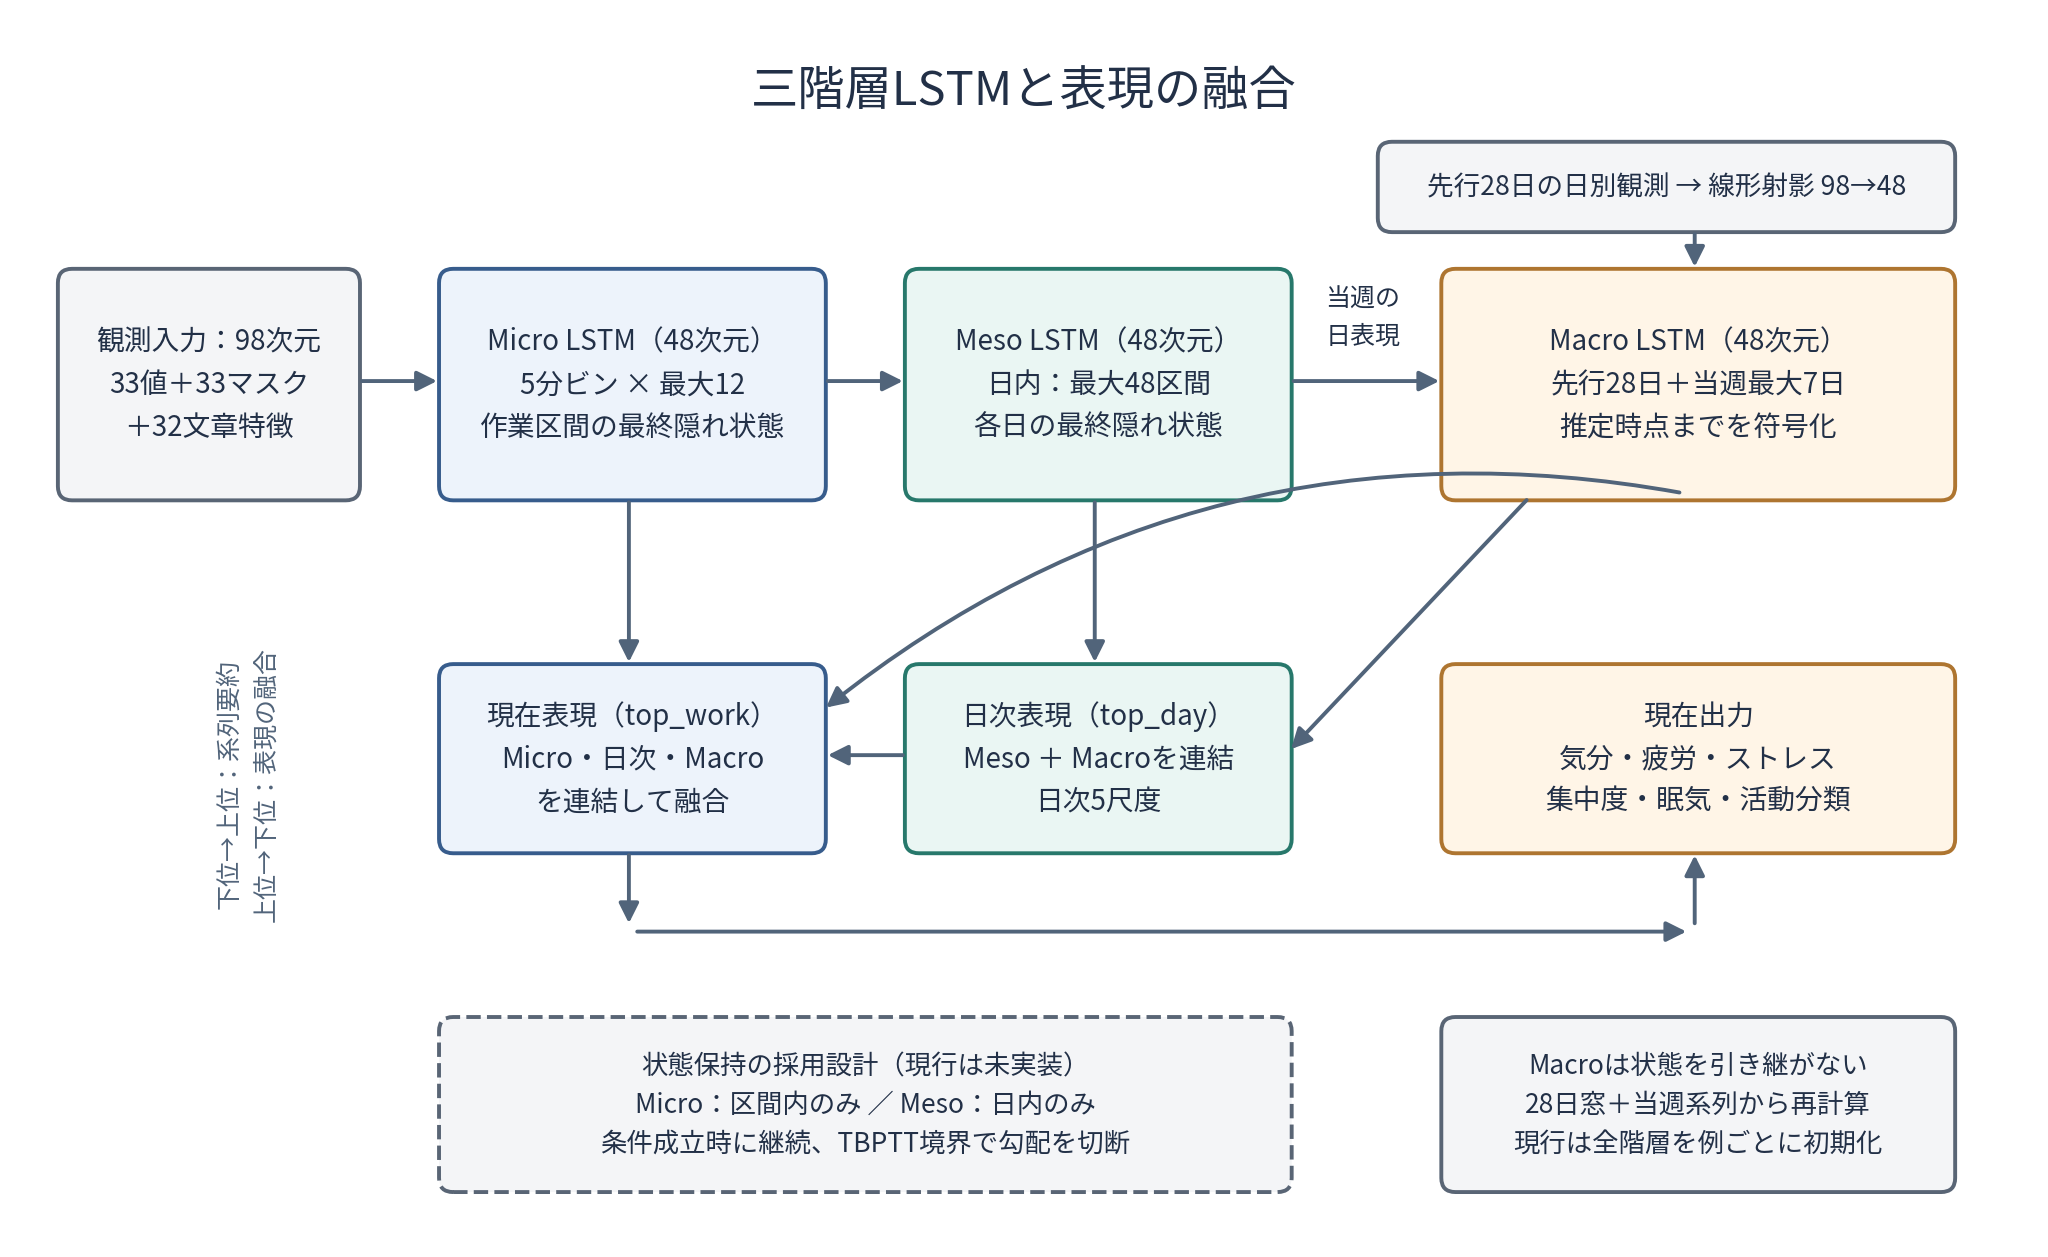
\includegraphics[width=\linewidth]{figures/fig_hierarchical_lstm.png}
  \caption{固定活動分類を持つ従来HierarchicalLSTMの図である。現在出力の「活動分類」は新方式には存在しない。下段の状態保持・TBPTTは従来の比較設計の注記であり、運用実装はいずれの方式でも系列ごとに初期化する。本図を新方式のPlace/Behavior射影と同時学習の検証資料として用いない。}
  \label{fig:legacy-lstm}
\end{figure}

従来の本人履歴条件付けは、本人の過去回答の平均を表現へ加える操作である。参加者\(p\)、予測時刻\(t\)、回答対象\(s\in\{\mathrm{cur},\mathrm{day}\}\)に対し、回答記録\(e\)の参加者を\(p_e\)、回答対象を\(s_e\)、対象時刻を\(t_e^{\rm target}\)、受信時刻を\(t_e^{\rm recv}\)、尺度\(j\)の回答を\(y_{ej}\)、有限かつ有効な回答が存在する指示を\(m_{ej}\in\{0,1\}\)とする。\(j=1,\ldots,5\)は§\ref{sec:prediction-targets}の尺度順序に対応する。全履歴、同時刻帯、同曜日、同活動の四群を表す群集合を\(\mathcal G\)とする。

\[
\mathcal G=\{\mathrm{all},\mathrm{hour},\mathrm{weekday},\mathrm{activity}\}.
\]

既存の群判定に従って回答\(e\)が時点\(t\)の群\(g\)に属するかを\(\chi_g(e;t)\in\{0,1\}\)とし、\(\chi_{\rm all}(e;t)=1\)とする。

同時刻帯は日本標準時の同じ時刻の「時」、同曜日は同じ曜日への一致である。\(\operatorname{hour}\)と\(\operatorname{weekday}\)をそれぞれ時と曜日を返す関数、\(a_e\)を回答\(e\)に対応する既存活動ID、\(a(t)\)を推定時刻までに利用可能な対象時点の既存活動IDとすると、

\[
\begin{aligned}
\chi_{\rm hour}(e;t)
&=\mathbf1\{\operatorname{hour}(t_e^{\rm target})=\operatorname{hour}(t)\},\\
\chi_{\rm weekday}(e;t)
&=\mathbf1\{\operatorname{weekday}(t_e^{\rm target})=\operatorname{weekday}(t)\},\\
\chi_{\rm activity}(e;t)
&=\mathbf1\{a(t)\text{が有効},\ a_e=a(t)\}.
\end{aligned}
\]

活動IDが未知のときは同活動群への一致を作らない。

\[
\begin{aligned}
\mathcal A_{pgj}^{s}(t)
&=\{e:p_e=p,\ s_e=s,\ t_e^{\rm target}<t,\
t_e^{\rm recv}<t,\ m_{ej}=1,\ \chi_g(e;t)=1\},\\
n_{pgj}^{s}(t)&=|\mathcal A_{pgj}^{s}(t)|,\qquad
\bar y_{pgj}^{s}(t)=
\frac1{n_{pgj}^{s}(t)}
\sum_{e\in\mathcal A_{pgj}^{s}(t)}y_{ej}
\quad\bigl(n_{pgj}^{s}(t)>0\bigr).
\end{aligned}
\]

四群は互いに排他的ではなく、一回答が複数群の平均に寄与してよい。件数が3件以上の群・尺度だけを有効とし、平均20個と存在指示20個を40次元特徴\(\phi_p^{s}(t)\)へまとめる。各群では5尺度の平均を先に、その後に5尺度の存在指示を並べ、四群をall、hour、weekday、activityの順に連結する。この順序は学習と推論で固定する。

\[
\begin{aligned}
v_{pgj}^{s}(t)&=\mathbf1\{n_{pgj}^{s}(t)\ge3\},\\
a_{pgj}^{s}(t)&=
\begin{cases}
\bar y_{pgj}^{s}(t),&v_{pgj}^{s}(t)=1,\\
3,&v_{pgj}^{s}(t)=0,
\end{cases}\\
\phi_p^{s}(t)&=
[a_{pg1}^{s}(t),\ldots,a_{pg5}^{s}(t),
v_{pg1}^{s}(t),\ldots,v_{pg5}^{s}(t)]_{g\in\mathcal G}
\in\mathbb R^{40},\\
P_p^{s}(t)&=\tanh(W_{\rm hist}\phi_p^{s}(t)+b_{\rm hist})
\in\mathbb R^{48},\\
C'^{\,s}&=C+P_p^{s}(t),\qquad D'^{\,s}=D+P_p^{s}(t).
\end{aligned}
\]

\(W_{\rm hist}\in\mathbb R^{48\times40}\)と\(b_{\rm hist}\in\mathbb R^{48}\)は履歴射影の学習パラメータであり、\(P_p^{s}(t)\)は履歴による条件付け表現である。補完値3は存在指示ゼロによって実測平均と区別する。current用とdaily用では利用する回答集合が異なるため、それぞれの履歴特徴を与えた順伝播から対応する出力層の値を採用する。一回の順伝播の内部では、同じ条件付け表現を現在・日次の双方へ加える。

同じ群判定の下で新たに利用可能となった回答値\(y\)を一件加えるとき、件数\(n\)と平均\(\bar y\)の更新は\(n^+=n+1\)、\(\bar y^+=\bar y+(y-\bar y)/n^+\)である。\(n=0\)なら\(\bar y^+=y\)で初期化する。ここで上付き\(+\)は追加後の統計を表す。この更新は回答統計の更新であり、モデル重みの更新ではない。予測時刻によって時刻帯等の群判定が変わる場合は、対象集合を選び直す。

条件付けは推論中の重み更新ではなく、過去56日の条件付きベースラインによる「普段との差」とも異なる。新方式ではこの40次元変換をモデルから除いている。従来基本モデルのパラメータ数86,050は固定24活動ヘッドと履歴条件付けを含む値であり、新方式のパラメータ数として用いない。

従来の教師損失は、活動例の交差エントロピーに係数0.2を掛け、現在または日次の尺度例には有効座標のHuber平均を用い、有効例間で平均する。活動例と尺度例を一例ごとに区別するこの集約は、§\ref{sec:joint-learning}の新方式で現在・日次の有効座標をそれぞれ平均する集約とは異なる。従来基本モデルはバッチ4、AdamW、学習率0.001・weight decay0.001、勾配ノルム上限1を用い、尺度の検証平均MAEで候補を選ぶ。

\subsection{従来構成：生観測GrowingMapと状態変更率}
\label{sec:legacy-transition-ratios}

従来GrowingMapはLSTMの隠れ状態をクラスタリングせず、10分の非重複打鍵窓から生観測特徴を作る。20 inserts以上の窓に対して挿入量の対数、訂正率、休止率、時刻の正弦・余弦を用いる。保存済み\texttt{context\_inference}のうち窓終端から10分以内で、受信が推定時刻に間に合い、拠点・Task両IDを持つ最も近い記録を対応させる。対応記録がなければラベルは未知とする。本人回答と文脈モデル推定の情報源を区別し、名称ではなく別名解決後の識別子で照合する。

観測座標集合\(O_z\)と中心\(i\)の観測座標集合\(O_i\)の共通部分\(J_i\)に対し、同じ拠点・Taskの識別子対を持ち、\(|J_i|\ge3\)の場合だけ

\[
d_i(z)=\sqrt{\frac1{|J_i|}\sum_{j\in J_i}(z_j-a_{ij})^2}
\]

を使い、それ以外は距離を\(+\infty\)とする。最小距離が半径\(\rho=0.35\)以内なら勝者へ割り当て、観測された座標だけを座標別回数\(n_{ij}\)による逐次平均で更新する。

\[
n'_{ij}=n_{ij}+1,\qquad
a'_{ij}=a_{ij}+\frac{z_j-a_{ij}}{n'_{ij}}\quad(j\in O_z).
\]

初めて観測した座標は回数1、値\(z_j\)とし、欠測座標は保持する。中心の接近による統合も座標別回数の加重平均で行い、同一ラベル・共通座標3以上・距離\(\rho/2\)以下を条件とする。古いIDを残し、削除IDを別名として解決し、端点を正規IDへ集約して自己辺を除く。これが従来構成の座標平均であり、新方式の正規化埋め込みの再帰更新とは異なる。

観測特徴が3以上で既存中心がないか距離が半径を超え、ノード数が256未満なら新ノードを生成する。上限到達後の遠い観測を最寄りへ強制割当しない。従来の状態変更回数と、その回数から導く構成比は

\[
\begin{aligned}
N_{ab}&\leftarrow N_{ab}+\mathbf1\{a\ne b,\ 0\le\Delta t\le12\text{時間}\},\\
Q_{ab}&=\frac{N_{ab}}{\sum_{c\ne a}N_{ac}}
\quad\left(b\ne a,\ \sum_{c\ne a}N_{ac}>0\right).
\end{aligned}
\]

である。\(Q_{ab}\)はAから記録された状態変更のうちBへ移った割合であり、Aへの滞在を含む次観測の遷移確率ではない。分母0なら未定義とし、保存対象は回数\(N_{ab}\)である。距離半径0.35と12時間の条件は新方式へ引き継がない。GrowingMapにも新方式にもGNGの誤差蓄積、第2勝者・近傍の更新、辺の加齢・削除則はなく、GNGの再現とは呼ばない\autocite{fritzke1995gng}。従来マップの処理図と詳細は§\ref{sec:legacy-growingmap}に示す。

\subsection{従来構成・比較計画：SSL、部分プーリングと逐次適応}
\label{sec:legacy-ssl-and-adaptation}

従来の\texttt{research/ssl.py}は、マスク再構成と5〜30分先の観測特徴予測で事前学習し、その後に固定活動分類・尺度の教師で微調整する二段階の実験経路である。マスク予測や再構成の一般的背景としてBERTとMasked Autoencodersを参照する\autocite{devlin2019bert,he2022mae}。従来SSLでは文章32座標のどれかを初期確率\(q=0.2\)で選んだ場合にブロック全体を隠すため、文章ブロックの選択確率は\(1-(1-q)^{32}\)である。新方式の最新ビンにおける文章ブロックの選択確率0.2とは異なる。

従来SSLは区間表現・日表現・Macro表現からの観測再構成、28日履歴再構成、将来予測のマスク付き二乗損失を係数1で合成する。将来教師のホライズンは5・10・15・20・25・30分から設定し、既定は5・15・30分である。SSL中は本人履歴をゼロ化し、固定活動・尺度ヘッド、履歴条件付け、個人バイアスを更新しない。事前学習後に補助ヘッドを外し教師付き学習へ進む。訓練カットオフより前の将来教師だけを使い、入力側のみから正規化統計を求める。§\ref{sec:joint-learning}の最新ビン再構成と次1時間予測を教師損失と同時に学ぶ構成へ、この旧機構を流用しない。

部分プーリングの独立実験経路\texttt{ExperimentalModel}は、実験内の共有エンコーダと参加者別の5次元バイアス\(b_p\)を用い、現在・日次に同じバイアスを加える\autocite{gelman2007multilevel}。参加者\(p\)の例\(e\)の観測入力を\(x_e\)、回答対象を\(s_e\)、尺度\(j\)の回答値を\(y_{ej}\)、回答マスクを\(m_{ej}\)とする。\(f_\theta^s(x_e)\in\mathbb R^5\)は共有重み\(\theta\)による回答対象\(s\)の尺度出力、\(n_{pj}\)は初期訓練および当該逐次更新までに取り込んだ参加者\(p\)・尺度\(j\)の回答数である。\(\tau>0\)はガウス事前の標準偏差、\(I\)は5次元単位行列、\(\lambda_b=10\)は収縮係数を表す。

\[
\begin{aligned}
\hat y_{p,e}^{s}&=f_\theta^{s}(x_e)+b_p,\qquad
b_p\sim\mathcal N(0,\tau^2I),\\
\ell_e^{\rm pool}
&=\frac1{\sum_{j=1}^5m_{ej}}
\sum_{j=1}^5m_{ej}
\left[
(f_\theta^{s_e}(x_e)_j+b_{pj}-y_{ej})^2+
\frac{\lambda_b b_{pj}^2}{\max(n_{pj},1)}
\right],
\quad \sum_{j=1}^5m_{ej}>0.
\end{aligned}
\]

ガウス事前は収縮罰則の解釈であり、事後分布を計算する実装ではない。尺度損失はHuberではなく二乗誤差で、活動には係数0.2付き交差エントロピーを用いる。参加者バイアスへのAdamW weight decayはゼロとし、明示的な収縮を二重適用しない。シグモイド出力後にバイアスを加えるため、出力は1〜5を超え得て、現行実験ではクリップしない。未登録参加者のバイアスはゼロとする。全参加者共通の完成済みグローバルモデルが配布されていることを前提とせず、新方式へ部分プーリングを追加済みとも解釈しない。

prequential比較では、各参加者の予測値と更新に用いた回答数を、対象の回答を受信する前に保存し、その後届いた教師で採点する。参加者\(p\)の予測時刻列を\(t_1<t_2<\cdots\)、時刻\(t_k\)で過去回答による更新を行う前の参加者内モデル重みを\(\theta_{p,k,0}\)、観測入力を\(x_p(t_k)\)とする。\(\mathcal U_{p,k}\)はそれまでの逐次更新に使った回答ID集合であり、最初は空集合とする。参加者内モデルの初期訓練締切を\(T_p^{\rm tr}\)とし、初期訓練期間の回答を再び新規教師として使わない。更新用回答集合\(\mathcal A_{p,k}\)には、締切以後の対象時刻で、予測より厳密に前に対象時刻と受信時刻の双方があり、まだ更新に使っていない有効回答だけを含める。

\[
\begin{aligned}
\mathcal A_{p,k}
&=\{e:p_e=p,\ T_p^{\rm tr}\le t_e^{\rm target}<t_k,\ t_e^{\rm recv}<t_k,\
\mathrm{id}_e\notin\mathcal U_{p,k},\ e\text{が有効教師例}\}.
\end{aligned}
\]

ここで\(p_e\)、\(\mathrm{id}_e\)、\(t_e^{\rm target}\)、\(t_e^{\rm recv}\)は回答の参加者、識別子、対象時刻、受信時刻を表す。この集合を受信順に並べ、同時刻の場合は対象時刻等の保存キーで順序を固定して、回答を一件ずつ更新へ用いる。予測後に到着した回答は時刻\(t_k\)の更新集合へ遡って追加せず、以後の予測時点で条件を満たしたときに利用する。

従来参加者内モデルの全層微調整では、活動例と尺度例を区別した損失\(\ell_e^{\rm online}\)を用いる。活動例の正解カテゴリを\(a_e\in\{1,\ldots,24\}\)、予測確率を\(\pi_{e,a_e}\)、尺度例の回答対象を\(s_e\)、有効尺度数を\(M_e=\sum_{j=1}^5m_{ej}\)とする。\(\rho_1\)は§\ref{sec:scale-and-total-loss}の閾値1のHuber関数である。

\[
\ell_e^{\rm online}=
\begin{cases}
-\log\pi_{e,a_e},&e\text{が活動例},\\
\displaystyle\frac1{M_e}\sum_{j=1}^5
m_{ej}\rho_1(\hat y_{ej}^{s_e}-y_{ej}),
&e\text{が尺度例},\ M_e>0.
\end{cases}
\]

\(\mathcal A_{p,k}\)を並べた列を\((e_1,\ldots,e_{R_{p,k}})\)、その長さを\(R_{p,k}=|\mathcal A_{p,k}|\)とする。回答\(e_r\)を使う直前の重みは\(\theta_{p,k,r-1}\)である。勾配\(g_{p,k,r}=\nabla_{\theta_{p,k,r-1}}\ell_{e_r}^{\rm online}\)を計算する。勾配ノルムの上限1に合わせて\(\operatorname{clip}_1(g)=g/\max(1,\|g\|_2)\)と定義し、一件ごとの更新と予測保存を次式で表す。

\[
\begin{aligned}
\theta_{p,k,r}
&=\operatorname{AdamW}_{\eta}(\theta_{p,k,r-1},\operatorname{clip}_1(g_{p,k,r})),
\quad
\eta=0.0001,\quad r=1,\ldots,R_{p,k},\\
\hat y_{p,k}
&=f_{\theta_{p,k,R_{p,k}}}(x_p(t_k)),\qquad
\theta_{p,k+1,0}=\theta_{p,k,R_{p,k}},\\
\mathcal U_{p,k+1}
&=\mathcal U_{p,k}\cup\{\mathrm{id}_e:e\in\mathcal A_{p,k}\}.
\end{aligned}
\]

\(\operatorname{AdamW}_{\eta}\)は当該参加者の最適化状態を保持する学習率\(\eta\)のAdamW更新を表す。活動交差エントロピーには通常学習の係数0.2を掛けない。更新集合が空なら重みと使用済みID集合を保持する。保存した\(\hat y_{p,k}\)を後の重みで再計算しない。参加者\(p\)の回答で他参加者の従来参加者内モデルを更新しない。

この更新演算を明示するため、参加者\(p\)の通算更新番号を\(q\ge1\)とし、その更新に対応するノルム制限後の勾配を\(\bar g_{p,q}=\operatorname{clip}_1(g_{p,k,r})\)、更新後の重みを\(\theta_p^{(q)}\)と書く。勾配の一次・二次モーメントを\(m_{p,q}^{\rm opt},v_{p,q}^{\rm opt}\)とし、初期値はともに0である。\(\beta_1,\beta_2\in[0,1)\)はモーメントの減衰係数、\(\epsilon_{\rm opt}>0\)は分母の安定化定数、\(\lambda_{\rm wd}\ge0\)はweight decay係数であり、最適化の設定として記録する。AdamW演算は

\[
\begin{aligned}
m_{p,q}^{\rm opt}
&=\beta_1m_{p,q-1}^{\rm opt}+(1-\beta_1)\bar g_{p,q},\\
v_{p,q}^{\rm opt}
&=\beta_2v_{p,q-1}^{\rm opt}
+(1-\beta_2)(\bar g_{p,q}\odot\bar g_{p,q}),\\
\hat m_{p,q}^{\rm opt}
&=\frac{m_{p,q}^{\rm opt}}{1-\beta_1^q},\qquad
\hat v_{p,q}^{\rm opt}=\frac{v_{p,q}^{\rm opt}}{1-\beta_2^q},\\
\theta_p^{(q)}
&=(1-\eta\lambda_{\rm wd})\theta_p^{(q-1)}
-\eta\frac{\hat m_{p,q}^{\rm opt}}
{\sqrt{\hat v_{p,q}^{\rm opt}}+\epsilon_{\rm opt}}
\end{aligned}
\]

である。\(\hat m^{\rm opt},\hat v^{\rm opt}\)は初期値0による偏りを補正したモーメントであり、平方根とベクトル間の除算は座標ごとに行う。モーメントと通算番号\(q\)は予測時点が変わっても保持する。weight decayは適応的な勾配項と別に重みへ作用するため、損失へ二乗罰則を足す更新と区別する。

部分プーリングのFrozen・Biasのみ適応・全層適応の三条件は別経路である。比較条件ごとに共有重みと全参加者のバイアスを独立に複製し、そのパラメータを\(\psi=(\theta,\{b_p\}_p)\)とする。この経路では使用済み集合を初期訓練例のキーで初期化し、対象時刻・受信時刻が予測より厳密に前という条件と、未使用という条件で回答を選ぶ。参加者内モデルの対象時刻下限をそのまま追加せず、初期訓練で未使用の遅延回答も利用条件で判定する。共有モデルの比較では参加者ごとの回答を同じ受信順の列へまとめる。回答\(e\)による更新の直前と直後のパラメータを\(\psi^{-},\psi^{+}\)とする。更新目的\(\ell_e^{\rm comp}\)には、尺度例なら\(\ell_e^{\rm pool}\)、活動例なら係数0.2付き交差エントロピーを用いる。更新する座標を選ぶ指示ベクトル\(v_e\)を用いると、

\[
\psi^{+}
=\psi^{-}-\eta\,\operatorname{clip}_1
\left(v_e\odot\nabla_{\psi^{-}}\ell_e^{\rm comp}\right)
\]

である。Frozenでは\(v_e\)の全座標を0、Biasのみ適応では回答者\(p_e\)の\(b_{p_e}\)の座標のみ1、全層適応では全学習パラメータの座標を1とする。同一学習率のSGDを用い、momentumとweight decayは加えない。Biasのみ適応では他参加者のバイアス行を保持し、全層適応では共有重みも変化する。使用済み回答のキーは参加者、回答ID、回答対象の組とする。これらは評価用の逐次適応条件であり、ライブ推論のオンライン学習を実装したという主張ではない。

適応条件では尺度回答\(e\)を損失へ渡す前に、回答者の件数を\(n_{p_ej}^{+}=n_{p_ej}^{-}+m_{ej}\)と更新し、収縮項の分母には追加後の件数を使う。上付き\(-,+\)は当該回答を取り込む直前・直後を表す。Frozen条件の件数と重みは保持する。

状態保持型TBPTTは独立の比較計画である\autocite{williams1990tbptt}。階層\(\ell\in\{\mu,m\}\)の系列を、最大\(L_\ell\)ステップのチャンクへ分ける。\(L_\mu\)はMicroの5分ビン数、\(L_m\)はMesoの区間表現数による切断長であり、\(1\le L_\mu\le12\)、\(1\le L_m\le48\)の整数とする。これらの上限は既存の系列上限から与えるもので、固定の既定切断長は現行本文・実装で定められていないため、比較実験の条件として両値を記録する。

階層\(\ell\)の有効系列長を\(J_\ell>0\)、チャンク番号を\(r=1,\ldots,\lceil J_\ell/L_\ell\rceil\)とすると、チャンク\(r\)の実際の長さは\(\min\{L_\ell,J_\ell-(r-1)L_\ell\}\)である。末尾の短いチャンクでは、有効系列の残りだけを処理する。

チャンク\(r\)の最終隠れ状態と最終セル状態を\(h_{\ell,r}^{\rm end},c_{\ell,r}^{\rm end}\in\mathbb R^{48}\)とする。\(r\)はチャンク番号であり、次チャンク冒頭への引継ぎ指示\(\gamma_{\ell,r}\in\{0,1\}\)が1である場合だけ、値を保存して勾配を切る。

\[
\begin{aligned}
(h_{\ell,r+1}^{\rm init},c_{\ell,r+1}^{\rm init})
&=
\begin{cases}
(\operatorname{stopgrad}(h_{\ell,r}^{\rm end}),
\operatorname{stopgrad}(c_{\ell,r}^{\rm end})),
&\gamma_{\ell,r}=1,\\
(0,0),&\gamma_{\ell,r}=0,
\end{cases}\\
\frac{\partial h_{\ell,r+1}^{\rm init}}
{\partial h_{\ell,r}^{\rm end}}&=0,\qquad
\frac{\partial c_{\ell,r+1}^{\rm init}}
{\partial c_{\ell,r}^{\rm end}}=0.
\end{aligned}
\]

\(\operatorname{stopgrad}\)は数値を保持し、前チャンクへの勾配だけを遮断する演算である。Microでは同一参加者・モデル版・日・作業区間の連続処理、Mesoでは同一参加者・モデル版・日内の連続処理に限って\(\gamma_{\ell,r}=1\)とする。Microは作業区間を処理するセッションの境界で、Mesoは日付境界で初期化する。ここでセッションとはモデルが処理する同一作業区間を指し、端末から届く個々のキーボードsession記録の境界とは区別する。参加者変更、意味境界、長い欠測、モデル版変更、処理時刻の逆行ではいずれも初期化する。

チャンク終了時には、参加者、モデル版、階層、対象の日・区間等を識別するキー、最終処理時刻、隠れ状態、セル状態を組として保存する。モデル版を\(\nu_{\rm model}\)とし、キーを\(\kappa_\mu=(p,\nu_{\rm model},\mu,d,u)\)、\(\kappa_m=(p,\nu_{\rm model},m,d)\)とする。チャンク\(r\)の最終処理時刻を\(t_{\ell,r}^{\rm end}\)とすれば、保存記録は

\[
\mathsf S_{\ell,r}=
(\kappa_\ell,t_{\ell,r}^{\rm end},
\operatorname{stopgrad}(h_{\ell,r}^{\rm end}),
\operatorname{stopgrad}(c_{\ell,r}^{\rm end}))
\]

である。復元はキーの一致と最終時刻より後の連続処理を確認した場合に限り、同じ観測を再処理して状態へ二重に取り込まない。区間終端ではMicroの保存状態を、日付終端ではMicro・Meso双方の保存状態を破棄する。週境界も日付境界に含まれる。Macroは隠れ状態・セル状態を持ち越さず、先行28日と当週の日表現から各回再計算する。状態値の長い保持と、勾配を伝える長さ\(L_\ell\)は別の条件である。この設計は評価予定であり、現行のバッチ学習・凍結推論とは分ける。

\subsection{従来構成：ベースライン暫定推定と切替}

従来のコールドスタート対応は、受信済みの本人平均・前回値を暫定値として表示し、項目ごとの十分な検証を得た後でLSTMへ切り替える独立経路である。有効化設定は既定で無効であり、新方式の支持不足による尺度非表示に追加する機構ではない。項目\(j\)に対し、対象時刻\(t_e\)と受信時刻\(r_e\)が予測より厳密に前の有効回答集合\(A_j(t)\)から

\[
\begin{aligned}
B_j^{\rm mean}(t)&=\frac1{|A_j(t)|}\sum_{e\in A_j(t)}y_{ej},\qquad
B_j^{\rm last}(t)=y_{e^*j},\\
e^*&=\operatorname*{arg\,max}_{e\in A_j(t)}(t_e,r_e,\mathrm{id}_e).
\end{aligned}
\]

を求める。回答ゼロなら値を出さない。受信前に保存した予測の過去MAEで平均が厳密に優れるときだけ平均を使い、同点または採点不足なら前回値を使う。暫定値には\texttt{source=baseline}、\texttt{provisional=true}、予測方法と先行回答数を付す。

同じ時系列検証回答IDでLSTMと両基準を採点する。訓練数\(N_j^{\rm tr}\)、共通検証数\(N_j^v\)、検証日数\(D_j^v\)、LSTMのMAE\(L_j\)、本人平均・前回値のMAE\(M_j,P_j\)を使い、\(B_j=\min(M_j,P_j)\)とすると、

\[
Q_j=\mathbf1\{N_j^{\rm tr}\ge10,\ N_j^v\ge10,\ D_j^v\ge3\},\qquad
W_j=\mathbf1\{Q_j=1,\ L_j\le B_j-0.1,\ L_j\le0.9B_j\}
\]

である。新規回答を含む別日の適格勝利を3回連続して満たした場合に切り替え、同じ回答や同日の再評価では連続数を進めない。日付の隣接する3日を要求する規則ではない。切替後は受信前に保存した直近10件の表示予測と両基準を同一集合で比較し、LSTMが良い基準より0.1点以上悪いという新規回答を伴う別日の判定が2回連続した場合にベースラインへ復帰する。9件以下では復帰判定をしない。閾値は切替条件であり、改善結果ではない。

回答ID、モデル・分割ID、件数・日数、MAE、閾値、連続数、source変更と理由を監査ログへ追記する。過去の予測を現在の重みで再計算して採点を代用せず、同一予測への重複回答を件数へ加えない。候補モデルの昇格と表示の切替は別判断である。暫定疲労値は疲労増加判定・休憩提案の根拠から除く。

\subsection{従来構成：状態内歩数、支援提案とPMTT}

従来の運動提案は、累積歩数の差を後側観測のGrowingMap状態\(s\)へ帰属させ、同状態・同参加者・同端末の過去日と比較する。参加者と端末を固定し、観測\(i\)の累積歩数を\(P_i\)、観測時刻を\(t_i\)、割当て状態を\(z_i\)とする。利用集合\(V\)は同じ日の非減少累積値で、観測間隔\(t_i-t_{i-1}\)が900秒以下、前観測と保存済み状態の結合が有効な対の添字集合である。日\(d\)の状態\(s\)に属する歩数を\(S_{s,d}\)として、

\[
\Delta P_i=\max(0,P_i-P_{i-1}),\qquad
S_{s,d}=\sum_{\substack{i\in V:\\z_i=s,\ \operatorname{day}(t_i)=d}}
\Delta P_i
\]

と定義する。\(\operatorname{day}\)は日本標準時の日付を返す。長い欠測中の増分を最後の状態へ一括帰属しない。現在の計測・端末文脈にも900秒以内の鮮度を要求し、当日の正の歩数増分を携帯の根拠とする。

判定時刻\(t\)の当日を\(d_0=\operatorname{day}(t)\)とし、同じ参加者・端末・状態\(s\)・仕様版の有効基準日集合を\(\mathcal D_s(t)=\{d:d<d_0,\ d\text{が有効基準日}\}\)とする。対応する歩数の列を\(\mathcal B_s(t)=(S_{s,d})_{d\in\mathcal D_s(t)}\)とし、同じ歩数の日も日ごとに一件として保持する。状態の別名は正規IDへ解決してから集計する。\(n_s(t)=|\mathcal D_s(t)|\)は基準日数であり、零歩も有効に計測された日には値として保持する。中央値\(m_s(t)\)と25パーセンタイル\(q_s(t)\)を次式で定義する。

\[
m_s(t)=\operatorname{median}\mathcal B_s(t),\qquad
q_s(t)=Q_{0.25}(\mathcal B_s(t)).
\]

\(Q_{0.25}\)は実装と同じ線形補間による標本分位点演算であり、\(q_s\)は状態\(s\)の過去日の歩数の下位25\%に対応する基準である。具体的には、昇順に並べた\(n\)個の値を\(b_{(1)},\ldots,b_{(n)}\)、分位を\(\alpha\in[0,1]\)とし、\(\xi=(n-1)\alpha\)、\(j=\lfloor\xi\rfloor+1\)、\(\lambda=\xi-\lfloor\xi\rfloor\)とおけば、\(Q_\alpha=(1-\lambda)b_{(j)}+\lambda b_{(\min(j+1,n))}\)である。\(\lfloor\cdot\rfloor\)は床関数であり、中央値も\(Q_{0.5}\)と一致する。空の列では基準を定義しない。現在までに集計された当日の歩数\(S_{s,d_0}(t)\)から、整数へ丸めた不足歩数\(D_s(t)\)と不足判定\(\mathrm{low}_s(t)\in\{0,1\}\)を求める。

\[
\begin{aligned}
D_s(t)&=\operatorname{round}
\bigl(\max\{0,m_s(t)-S_{s,d_0}(t)\}\bigr),\\
\mathrm{low}_s(t)&=
\mathbf1\{S_{s,d_0}(t)<q_s(t),\
D_s(t)\ge500,\ D_s(t)\ge0.25m_s(t)\}.
\end{aligned}
\]

\(\operatorname{round}\)は最近接整数への丸めで、等距離の場合は偶数を選ぶ。\(\mathbf1\)は条件が真のとき1となる指示関数である。三条件はすべて同時に要求する。\(n_s(t)<3\)なら判定せず、3〜4日は暫定、5日以上を正式とする。同一時間帯まで揃えた比較ではなく、当日途中と過去日の値を比較する機構である。判定条件と、歩数・携帯根拠の鮮度条件を満たした場合にのみ換算へ進む。

不足歩数を100歩/分の仮定で歩行相当時間へ変換し、参照METsの比を用いて候補活動\(a\)の時間を求める\autocite{ainsworth2011compendium,tudorlocke2019cadence}。\(T_{\rm walk}\)は歩行相当時間、\(T_a\)は丸め前の活動時間、\(\tilde T_a\)は提示する活動時間であり、いずれも単位は分である。\(\mathrm{METs}_a>0\)は活動\(a\)の参照METs値、3.0は参照歩行のMETs値とする。

\[
\begin{aligned}
T_{\rm walk}&=\frac{D_s(t)}{100},\\
3.0\,T_{\rm walk}&=\mathrm{METs}_a\,T_a,\qquad
T_a=T_{\rm walk}\frac{3.0}{\mathrm{METs}_a},\\
\tilde T_a&=\max\left(5,5\left\lceil T_a/5\right\rceil\right).
\end{aligned}
\]

\(\lceil\cdot\rceil\)は天井関数であり、活動時間は最小5分、5分単位で切り上げる。第2式はMETsと時間の積を揃える換算の仮定を明示する。実装の参照表は歩行3.0、速歩4.3、階段上り8.0、自転車6.8、ジョギング7.0、ストレッチ2.3、ラジオ体操4.0であり、既定では先頭4件を最大4候補として返す。換算は本人固有の消費エネルギーを推定するものではない。状態統合の別名解決と仕様版を保持し、異なる版の基準を混ぜない。歩数取得への同意と運動提案の有効化は独立であり、運動提案は既定で無効である。

従来の休憩提案\texttt{breakCheck}は疲労の高さ・持続的増加、または入力訂正の変化と本人の「誤入力」という確認を候補根拠とする。訂正の増加だけで疲労と断定しない。運動・休憩提案には時間帯、予定中抑止、質問間隔、日上限、停止・延期の提示条件を適用し、受諾、実行、有用性を別に記録する。現行の共通キューでは、イベント提案の選択には質問予算を4枠より増やす必要があり、提案スイッチだけをONにしても既定4枠で自動発行されるわけではない。参加者内の提示・非提示の無作為割付は追加実装を必要とする評価計画である。

PMTTは観測、推定、根拠、本人修正を分離する従来の情報設計であり、発見モデル自体ではない。概念上の四要素を\(M_{p,t}=(O_{p,t},I_{p,t},E_{p,t},R_{p,t})\)とする。\(O\)は観測、\(I\)は当時のモデルによる推定、\(E\)は推定・提案を支持する根拠、\(R\)は本人の回答・修正を表す。これらの情報と時間枠を結ぶ有向グラフを\(\mathcal G_{\rm PMTT}=(\mathcal V_{\rm PMTT},\mathcal E_{\rm PMTT})\)とし、\(\mathcal V_{\rm PMTT}\)を記録・時間枠・提案の頂点集合、\(\mathcal E_{\rm PMTT}\)を関係型を持つ辺の集合とする。

観測記録の頂点を\(o\)、推定を\(i\)、根拠を\(e\)、本人回答・修正を\(r\)、提案を\(a\)とする。また、観測\(o\)の発生時刻を含む正時区間の頂点を\(u(o)\)、その日の頂点を\(d(o)\)、月曜起点の固定週の頂点を\(w(o)\)とする。概念上の主要な接続は、

\[
\begin{aligned}
o&\xrightarrow{\rm used\ by}i,\qquad
e\xrightarrow{\rm supports}i\ \text{または}\ a,\qquad
r\xrightarrow{\rm targets}i\ \text{または}\ u(o),\\
o&\longrightarrow u(o)\longrightarrow d(o)\longrightarrow w(o)
\end{aligned}
\]

である。第1行は推定・提案の由来と修正の対象を表し、第2行はObservation、StateEpisode、Day、固定週Patternという時間枠間の階層的な所属を表す。時間枠間の辺と、§\ref{sec:pattern-discovery}のBehaviorプロトタイプ間の時間遷移辺は役割が異なる。時間枠の頂点は観測を整理する区間であり、プロトタイプの頂点は類似した表現をまとめる状態である。

従来APIは\texttt{session}、\texttt{narrative}、\texttt{correction}、\texttt{inference}等を情報源属性の異なるObservationとして包む。運動提案はExerciseProposalと\texttt{supports}関係に状態ID・仕様版、通常値、今日値、不足、基準日数、観測ID、携帯根拠とMETs換算を保持する。四種の専用ノードと全推定の完全な依存グラフを実装したという意味ではない。

修正頂点\(r_{\rm new}\)と対象への辺を加える操作は、頂点・辺集合の追記\(\mathcal V_{\rm PMTT}^{+}=\mathcal V_{\rm PMTT}\cup\{r_{\rm new}\}\)、\(\mathcal E_{\rm PMTT}^{+}=\mathcal E_{\rm PMTT}\cup\{(r_{\rm new},{\rm targets},i)\}\)と表せる。上付き\(+\)は修正追加後を表し、対象が区間の場合は辺の終点\(i\)をその区間頂点へ置き換える。元観測と当時の推定は保持する。この役割分離は、新方式でも確認・命名・訂正と再解析の扱いに継承する。一方、従来の状態内歩数と介入の根拠を新しいBehavior IDへ検証なしに接続しない。PMTTの情報モデルを保持することと、新方式による支援効果の実証は別の課題である。
